 \documentclass[structabstract]{aa}

\usepackage{natbib}
\usepackage{graphicx}
\usepackage{epstopdf}
\usepackage{color}
\usepackage{hyperref}
\hypersetup{colorlinks, citecolor=blue, filecolor=black, linkcolor=black, urlcolor=black}


\newcommand{\vdag}{(v)^\dagger}
\newcommand{\myemail}{jbyrne@ifa.hawaii.edu}

%%I'm adding these -JPB
%\newcommand{\solphys}{{\it Solar Physics}}
%\newcommand{\aap}{    {\it Astronomy \& Astrophysics}}
%\newcommand{\aaps}{   {\it Astronomy \& Astrophysics Supplemental}}
%\newcommand{\apj}{    {\it Astrophysical Journal}}
%\newcommand{\apjl}{    {\it Astrophysical Journal Letters}}
%\newcommand{\jgr}{    {\it Journal of Geophysical Research}}
%\newcommand{\aapr}{    {\it Astronomy \& Astrophysics Review}}
%\newcommand{\grl}{    {\it Geophysical Research Letters}}
\newcommand{\lrsp}{    {\it Living Rev. Solar Phys.}}
\newcommand{\stat}{Ann. Stat.}

\newcommand{\RNum}[1]{\uppercase\expandafter{\romannumeral #1\relax}}

\usepackage{subfigure}

%\makeatletter
%\newcommand*{\rom}[1]{\expandafter\@slowromancap\romannumeral #1@}
%\makeatother


\begin{document}

\title{Numerical methods for determining the kinematics of CMEs and ``EIT Waves''}

\author{J.P.~Byrne\inst{1}
	\and D.M.~Long\inst{2}
	\and P.T.~Gallagher\inst{3}
	\and S.A.~Maloney?\inst{4}
	\and S.D.~Bloomfield?\inst{3}
	\and H.~Morgan\inst{5,1}
	\and S.R.~Habbal\inst{1}}
\institute{Institute for Astronomy, University of Hawai'i, 2680 Woodlawn Drive, Honolulu, HI 96822, USA.\\
		\email{jbyrne@ifa.hawaii.edu}
		\and
		UCL--Mullard Space  Science Laboratory, Holmbury St. Mary, Dorking, Surrey, RH5 6NT, UK.
		\and 
		School of Physics, Trinity College Dublin, College Green, Dublin 2, Ireland.
		\and
		Skytek, 51/52 Fitzwilliam Square West, Dublin 2, Ireland
		\and
		Institute of Mathematics and Physics, Aberystwyth University, Ceredigion, SY23 3BZ, UK.
		}

\date{Received ?; accepted ?}
%%Abstract
\abstract
% Context (optional)
{\emph{Why are we doing this work?} }
% Aims (mandatory)
{In this paper we show that traditional techniques for the determination of CME and ``EIT wave'' kinematics, as currently applied, do not return accurate estimates of the true kinematics of the feature. We highlight the errors inherent in these approaches and illustrate a recipe for accurate estimates of the kinematics using a residual resampling bootstrapping approach to determine the confidence interval associated with the model used to measure them.}
% Methods (mandatory)
{We discuss the errors inherent in the use of numerical differentiation techniques when applied to small data--sets. We present a residual resampling bootstrapping approach as a statistically rigorous technique for the determination of accurate kinematic estimates.}
% Results (mandatory)
{It is shown that accurate feature kinematics can only be estimated by applying a pre--determined model to the position measurements. The validity of this model must be based on the physical properties of the feature that are to be measured, and the accuracy of applying that model to the data can be examined using a bootstrapping approach to determine the confidence interval associated with the estimated model parameters.}
% Conclusions (optional)
{\emph{What are our conclusions?}}

%% Keywords 

\keywords{Sun: activity -- Sun: corona -- Sun: coronal mass ejections (CMEs)}

\maketitle

%
%________________________________________________________________

\section{Introduction}
\label{sect_intro}

% Set the scene
The most defining feature of a transient solar phenomenon such as a Coronal Mass Ejection (CME) or a coronal wave (commonly called an ``EIT Wave'') is its motion. These generally short--lived features, resulting from a solar eruption, are observed to propagate across the solar corona (i.e., coronal waves) or in the case of CMEs, outward from the Sun into the heliosphere. 
Observational catalogues of both phenomena have been compiled over more than $\sim$20~years of observations \citep[e.g.,][]{1985JGR....90..275I,2004JGRA..10907105Y,2009ApJS..183..225T}, with the physical properties of both phenomena very well characterised \citep[see the recent reviews by e.g., ][]{2011SSRv..158..365G,2012SoPh..tmp...93P,2011ASSL..376.....H,2012LRSP....9....3W}. 

% We're interested in motion here
As transient phenomena, the kinematics of both sets of features continue to be one of the most important characteristics used to classify them. The motion of both phenomena is traditionally identified using difference images, where a preceding image is subtracted from a leading image to highlight motion, allowing the feature to be identified ``by eye''. However, this approach highlights \emph{relative} rather than \emph{actual} motion, and is prone to undefined user--dependent bias. More recent work has used single image processing techniques such as wavelet transforms \citep{2009A&A...495..325B,2012ApJ...752..144M} and automated approaches \citep[e.g.,][]{2011A&A...531A..42L,2012ApJ...752..145B,2012SoPh..276..479P} to minimise user--error and reveal the true physical characteristics of the feature. By tracking the position of the feature with time it is possible to determine its kinematics, allowing an insight into the physical properties of the phenomenon. 

% Why we care about kinematics
The kinematics of these features are important for a variety of reasons. The true physical nature of coronal waves is not fully understood, with two main competing theories; that they are waves \citep[e.g.,][]{2012ApJ...754....7S,2010ApJ...716L..57V} or signatures of magnetic field restructuring during a CME eruption \citep[e.g.,][]{2011ApJ...738..167S,2011ApJ...732L..20C}. The kinematics of the feature have been proposed as one of the main discriminators between these competing theories, with the relatively high velocities measured thus far for this phenomenon suggesting a wave interpretation may be appropriate \citep[cf.][]{2011A&A...532A.151W,2012ApJ...753..112Z}. Similarly, CME kinematics are vitally important from a space weather point of view as they allow increased accuracy in the predicted arrival time of the feature at Earth. The kinematic behaviour of the CME very low down in the solar corona may also be used to discriminate between eruption mechanisms \citep[cf.][]{2010A&A...516A..44L}. However \citet{2007ApJ...657.1117W} demonstrate that the errors in CME acceleration values can be of the same order as the accelerations typically measured. 

% The step from distance-time to kinematics
A variety of different mathematical techniques exist for deriving the kinematics of transient features, ranging from the fitting of polynomial functions to the distance--time measurements to the numerical differentiation of the measurements. While these techniques may be mathematically sound, some of them are not necessarily applicable to the derivation of kinematics for these features and can produce spurious results. 




\begin{figure*}[!ht]
\centering
\subfigure{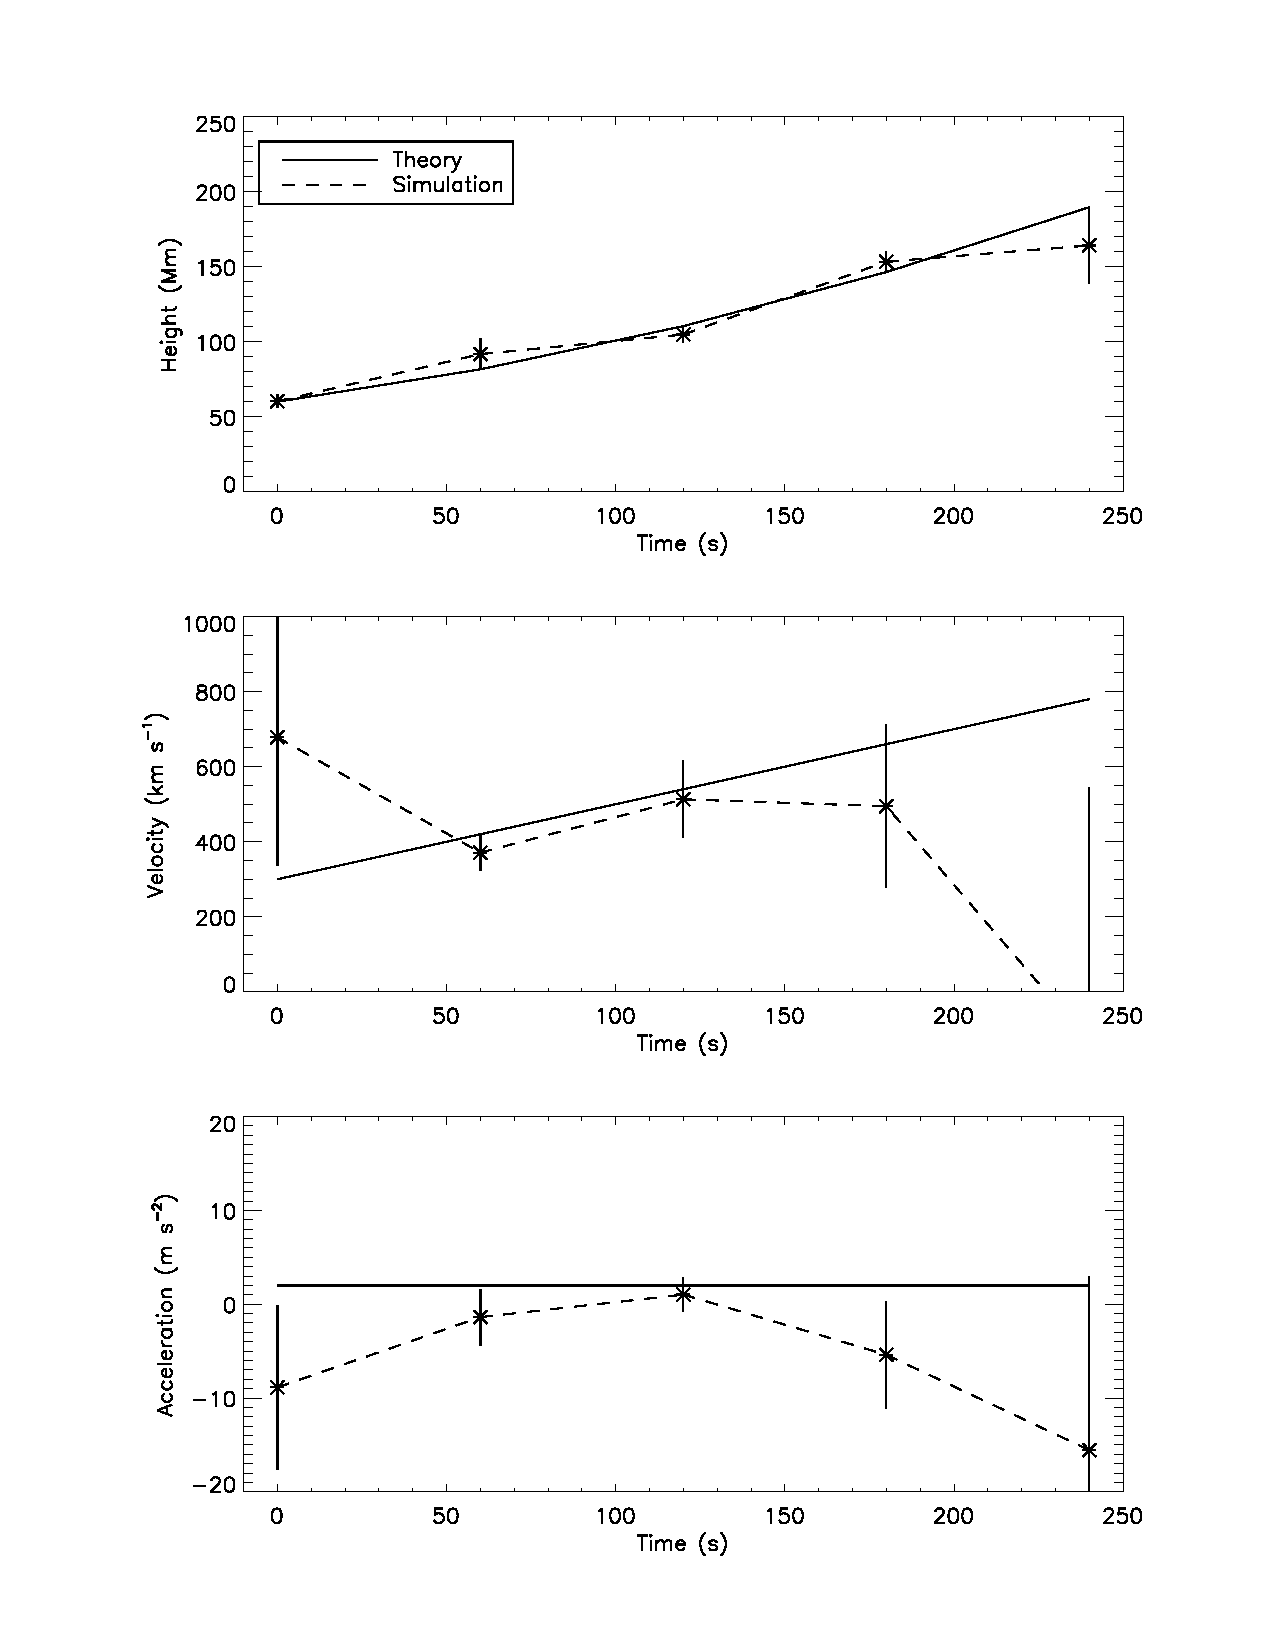
\includegraphics[scale=0.43, trim=110 50 70 70]{images/sim_vels_thesis1.pdf}}
\subfigure{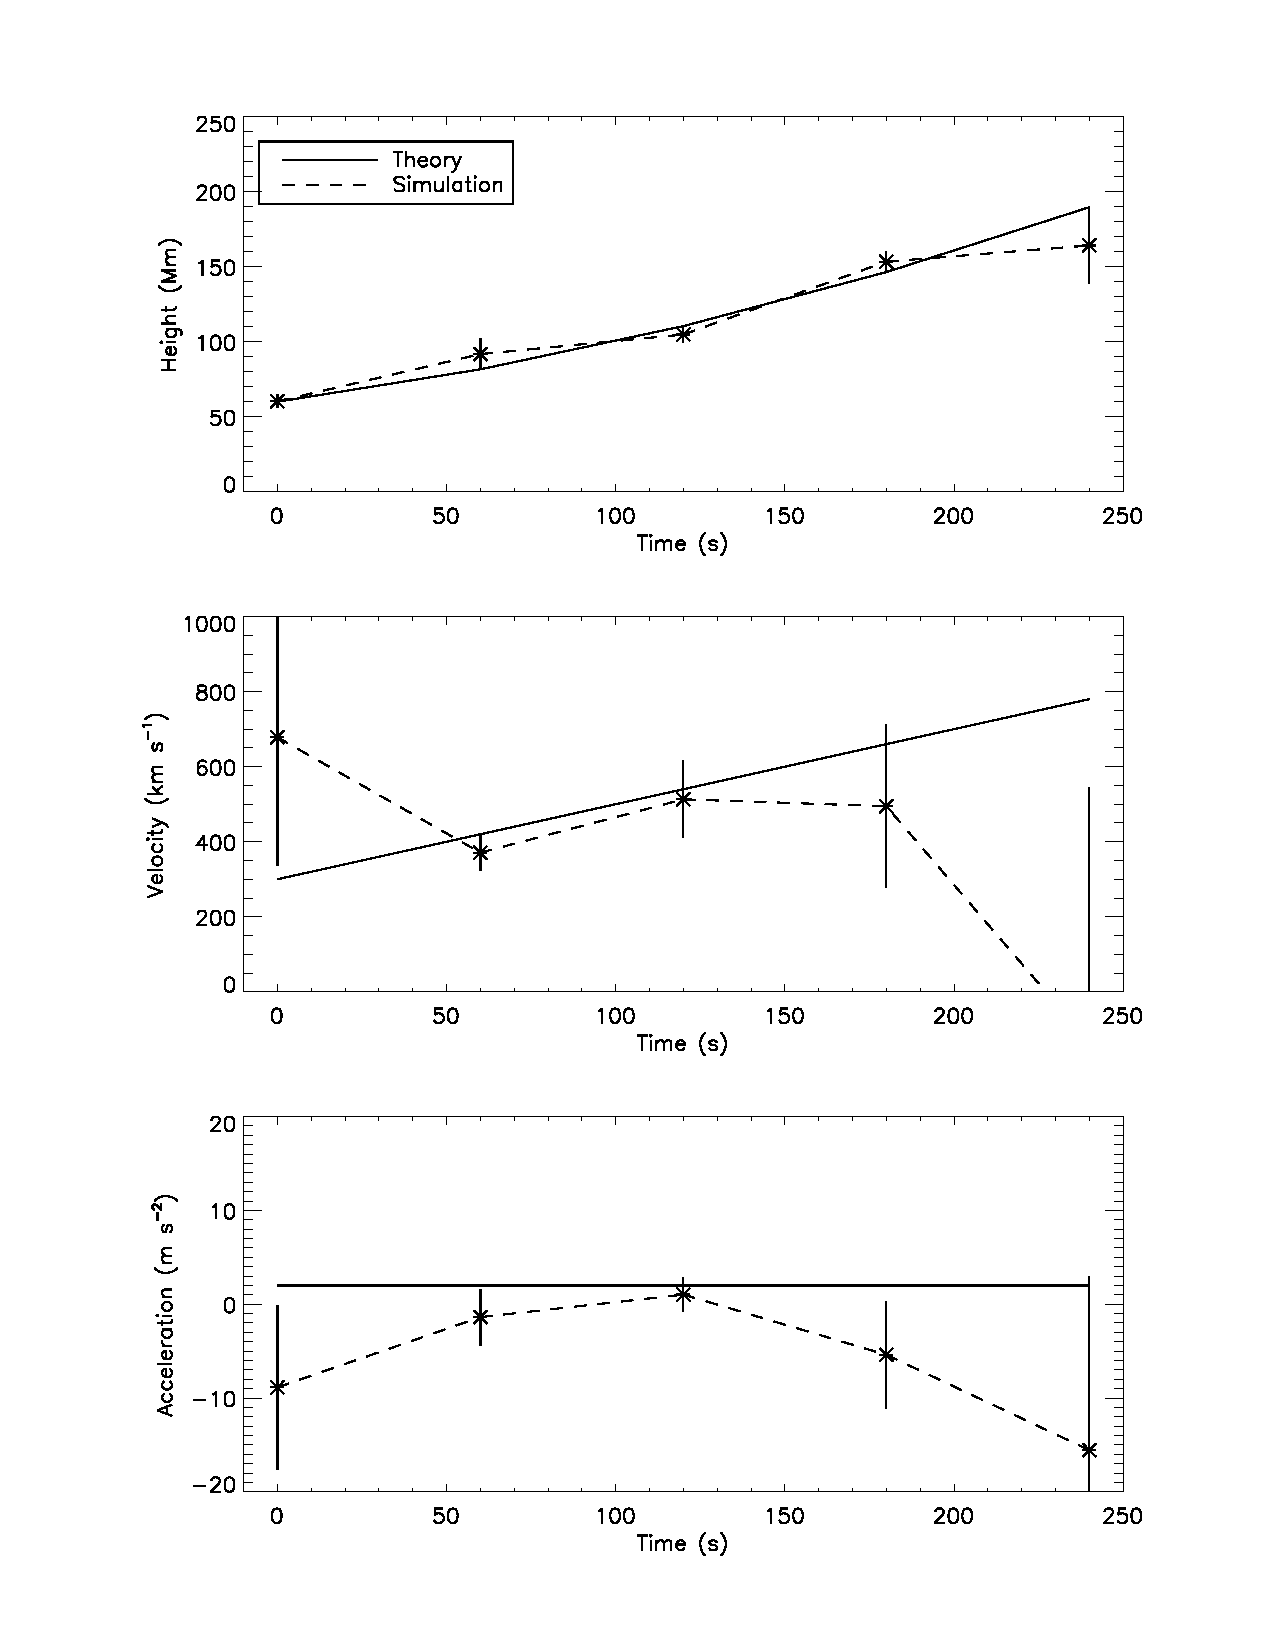
\includegraphics[scale=0.43, trim=70 50 110 70]{images/sim_vels_thesis2.pdf}}
\caption{A theoretical model for a CME with constant acceleration 2\,m\,s$^{-2}$ and initial velocity 300\,km\,s$^{-1}$, and two simulations of how the resulting profiles for a noisy sample of data--points behave using 3-point Lagrangian interpolation.}
\label{sim_vels_thesis}
\end{figure*}

\section{Numerical Differentiation \& Error Propagation (recap)}
\label{sect:num_diff_errors}

When presented with a moving object through a sequence of image frames such that it is possible to measure its position at each time step, the technique of numerical differentiation is often used to derive the velocity and acceleration of the object. In the standard 2-point approach, it should be possible to derive the time evolution of a system at time step $t+\delta t$ according to the system values at time step $t$. This may be applied through the technique of forward, reverse or centre differencing, resulting in an estimate of the speed of the object at a specific time step given its positional information. More commonly, a 3-point Lagrangian interpolation is applied to better approximate the kinematics of a moving object by solving for the Lagrange polynomials that best fit across three given datapoints (e.g. \textsc{deriv.pro} in IDL). Each of these schemes is based upon the Taylor series expansion of a real function $f(t)$:
\begin{equation}
\label{taylor1}
f(t_0+\delta t) \; = \; f(t_0)+f'(t_0)\delta t +  \frac{f''(t_0)}{2!}(\delta t)^{2}  + ...
\end{equation}
but due to the approximation of an infinite series with a finite number of terms and iterations, an error must be associated with the result, based on its deviation from the true solution. Generally the Euler method is employed, using the formula:
\begin{equation}
y_{n+1} \; = \; y_n + h f(t_n, y_n)
\end{equation}
to solve the initial value problem $y'=f(t,y)$ given $y(t_0)=y_0$, where $h$ is the stepsize such that $t_n=t_0+nh$. The convergence of such an approximation to the actual solution is prone to two sources of error; truncation error (the difference between the true solution and the approximation) and round-off error (the limited precision of the approximation). Added to this is the fact that the data measurements themselves are subject to uncertainties in both the positional and temporal information, and the ability of the numerical differentiation techniques to derive kinematics becomes highly jeopardised, as shall be shown.

Given a function $x=f(u,\,v)$, the error propagation equation (based on the standard deviations $\sigma$ of the variables) is written:
\begin{equation}
\label{eqn_errorprop}
\sigma_x^2 \; = \; \sigma_u^2 \left(\frac{\partial x}{\partial u}\right) ^2 + \sigma_v^2 \left( \frac{\partial x}{\partial v} \right) ^2 + 2 \sigma_{uv}^2 \left( \frac{\partial x}{\partial u} \right) \left( \frac{\partial x}{\partial v} \right) + ...
\end{equation}
Specifically in the case of kinematic analyses, this is used to propagate the errors on the distance-time data $r(t)$ into the velocity $v(t)$ and acceleration $a(t)$ profiles to determine the associated uncertainties. In the case of distance-time data the covariance terms are zero because the quantities are uncorrelated.

When presented with relatively low sampling of the data, as in the case of coronagraph observations of CMEs and disk observations of waves, it is generally found that the simplest differentiation techniques are not applicable. The forward and/or reverse differencing techniques act to shift the kinematic profiles by one time-step, which is substantial enough to be of concern here (i.e., they derive a result at the current time-step, based on the pro-/preceding time-step). Centre differencing employs the two neighbouring data-points of the point under examination, and so is a better indication of the result at that time-step, but it fails at both endpoints. In any case these should not be employed when the spacing of the data-points is unequal, i.e., when the cadence $\delta t$ is not constant, and so the 3-point Lagrangian interpolation technique is used (which gives the same result as the centre-difference otherwise, but includes the endpoints and has an associated error propagation formulation). The Lagrangian interpolation polynomial is given by:
\begin{eqnarray}
L(x) \; &=\; \sum_{j=0}^2 y_j l_j(x) \\ \quad \mbox{where} \quad
l_j(x) \; &=\; \prod_{i=0, i\neq j}^2 \frac{x-x_i}{x_j-x_i} 
\end{eqnarray}
The derivative at point $x$ is given by $L'=\partial_x L(x)$. So for the case of height-time data being used to derive velocity (and similarly acceleration) the associated error is given by:
\begin{equation}
\sigma_{v_1}^2 \,=\, \frac{\sigma_{r(t_2)}^2+\sigma_{r(t_0)}^2}{(t_2-t_0)^2} + v^2 \left( \frac{\sigma_{t_2}^2+\sigma_{t_0}^2}{(t_2-t_0)^2} \right)
\label{vel_err}
\end{equation}
with the endpoint errors derived from a weighting of the pro-/preceding two data--points, that is therefore larger to reflect the uncertainty of the trend beyond the sample points.

Although the 3-point Lagrangian is mathematically sound, its application to solar eruptive event kinematics proves problematic. The main drawbacks are two-fold:
\begin{enumerate}
\item The noise level across low-cadence measurements often belies the actual trends of the data, such that the numerical derivatives become untrustworthy and even misleading.
\item The error-propagation formulation results in a misleading uncertainty interval on the velocity and acceleration profiles, that for example counter-intuitively increases for increasing cadence measurements.
\end{enumerate}

Simulations of the drawbacks of a standard numerical derivative are presented in Section~\ref{sect:simul1}. In Section~\ref{sect:simul2} we outline a more appropriate method for inspecting the  kinematics of CMEs and waves, as applied to model data. In Section~\ref{sect:case_studies} some real-data cases are revisited with these methods, and motivate the proposed treatment of data from the new coronal image processing CME catalogue \citep[CORIMP;][]{2012ApJ...752..144M, 2012ApJ...752..145B}, and coronal pulse identification and tracking algorithm catalogue \citep[CorPITA;][]{2011A&A...531A..42L}. A final discussion and conclusions are presented in Section~\ref{sect:conclusions}.



\section{Simulations}
\label{sect:simul1}

In the case of CMEs and waves, there is great motivation to resolve the dynamics of their propagation as precisely as possible in order to study the forces at play. For example, CMEs in general may be undergoing continued driving (internal) forces, or positive or negative drag (external) forces, or most assuredly some interplay of both. Similarly wave propagation may be affected by changes to the low-coronal environs, e.g., low-density coronal hole regions. Thus any changes to event acceleration that result from different phases of dominating force, and where or why this can occur, are of great interest. But this all remains somewhat elusive given the inherent limitations of the data and the numerical methods employed.


\subsection{Effect of noise on the 3-point Lagrangian}
\label{subsect:test_lagrange_const}


As an example of drawback $1$ above, we simulate a simple distance-time profile of an event that propagates with a constant acceleration of 2\,m\,s$^{-2}$ and initial velocity 300\,km\,s$^{-1}$, and add random noise of various levels up to a maximum of 20\%. A `best case' errorbar on each datapoint is determined by its distance from the true height-time profile, to represent a scenario wherein all measurements lie on the very edge of the known error. Various instances of randomized datapoint scatters result in erroneous trends in the velocity and acceleration profiles - even with the proper error treatment ascribed by the 3-point Lagrangian interpolation technique. Two such cases are shown in Figure~\ref{sim_vels_thesis} where completely opposing acceleration trends are revealed, indicating that the nature of the scatter in the samples is not satisfactorily reflected in the derived kinematics and associated errors. The implication here is that if the sampling cadence is too low, the expected trends in the derived profiles will be completely intractable via these methods. One possible assurance is that instead of trusting the endpoints they simply be removed. Figure~\ref{sim_vels_thesis} would then show three datapoints for CME velocity and one datapoint for acceleration, that would go somewhat toward removing the biased trends and imply a constant acceleration close to the true value. This is especially of concern for fast-moving events that result in only a small number of distance-time measurements.


\subsection{Effect of cadence on the 3-point Lagrangian}
\label{subsect:test_lagrange_nonconst}


As an example of drawback 2 above, we simulate a non-constant acceleration profile via the following equations (as used in \citealt{2012ApJ...752..145B}):

\begin{eqnarray}
h(t)\,=&\,\sqrt{2x}\,t\tan^{-1}\left(\frac{e^{t/2x}}{\sqrt{2x}}\right) \\
v(t)\,=&\,\sqrt{2x}\tan^{-1}\left(\frac{e^{t/2x}}{\sqrt{2x}}\right)+\frac{e^{t/2x}t}{e^{t/x}+2x} \\
a(t)\,=&\,\frac{e^{t/2x}\left(2x\left(t+4x\right)-e^{t/x}\left(t-4x\right)\right)}{2x\left(e^{t/x}+2x\right)^2}
\end{eqnarray}

where the constant $x$ is just a scaling factor. The resulting acceleration profile exhibits an initial peak followed by a deceleration and then leveling to zero. This is akin to a general impulsive CME that undergoes an initial high-acceleration eruptive phase, and then decelerates to match the solar wind speed during its propagation phase. Thus a model CME height-time profile is generated enabling synthetic observation samples to be taken at different cadences (Figure~\ref{fig_cadence_hva}). 

\begin{figure*}[t]
\centering
\subfigure{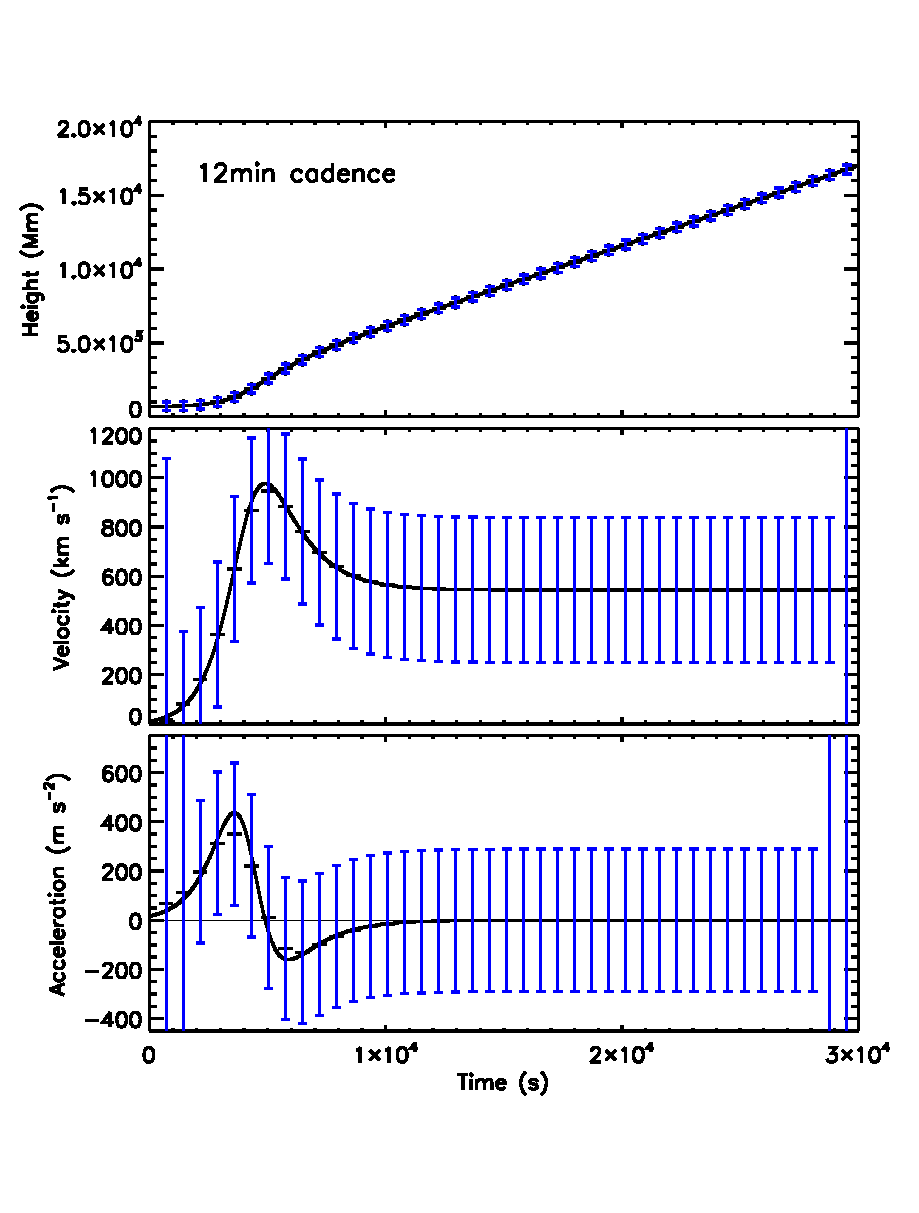
\includegraphics[scale=0.6, trim=0 55 0 50, clip=true]{images/fig_cadence_hva_12min.eps}}
\subfigure{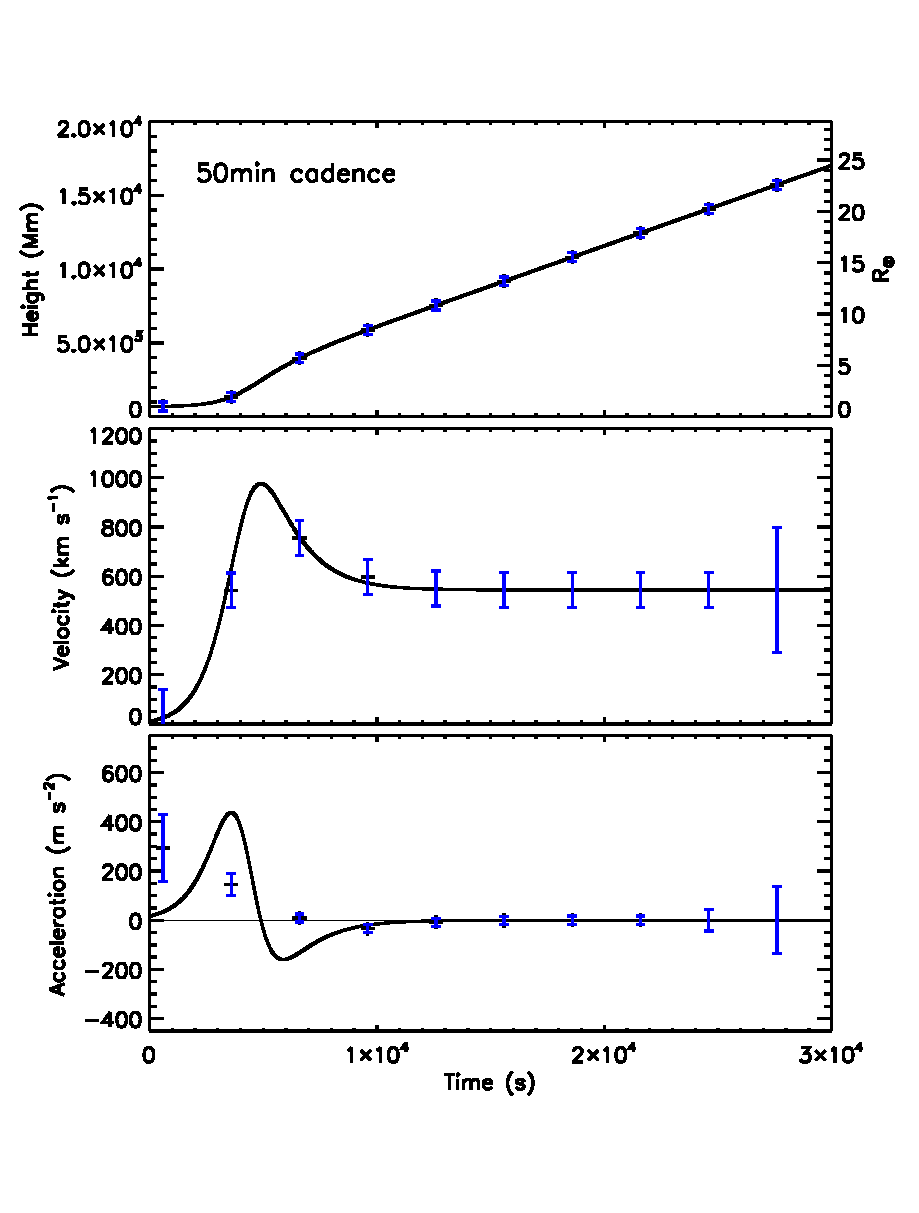
\includegraphics[scale=0.6, trim=0 55 0 50, clip=true]{images/fig_cadence_hva_50min.eps}}
\caption{A theoretical model for a CME with constant acceleration 2\,m\,s$^{-2}$ and initial velocity 300\,km\,s$^{-1}$, and two simulations of how the resulting profiles for a noisy sample of data--points behave using 3-point Lagrangian interpolation.}
\label{fig_cadence_hva}
\end{figure*}

We investigate the effect of the cadence of the observations on the derivation of the kinematics and associated errorbars using the standard 3-point Lagrangian interpolation. In the first instance fixed 3~$\sigma$ errorbars of $\pm$\,300\,Mm are applied to the height-time points, without any noise added. This is useful to simply test the effects of the cadence on the derived velocity and acceleration profiles and their associated errors. Figure~\ref{fig_cadence_4} shows a sample output of the test. Figures~\ref{fig_cadence_4}($a$) and ($b$) show the model CME acceleration profile sampled at cadences of 3 and 10~mins respectively, relative to the initial point at 0~mins (blue) held fixed while the varying cadence changes the locations of the other sample points along the profile. Note that the errorbars of the two points at both the start and end of the interval are larger than the rest to account for not having enough points to interpolate across them (the endpoints of velocity having already undergone the same treatment). As the cadence is reduced, i.e., the cadence time is increased, the errorbars become smaller due to the inverse dependence of the Lagrangian error treatment on the time between points ($\Delta t^{-2}$). However, reducing the cadence reduces the resolution with which it is able to detect the acceleration peak, and so the peak is smoothed out until the interval is eventually approximated as being one of constant zero acceleration, as demonstrated in Figure~\ref{fig_cadence_4}($d$) (where the non-smooth transition and errorbar sizes are as a result of stepping down in sample size such that the fixed point at 9~mins eventually becomes the start-point of the interval). Figure~\ref{fig_cadence_4}($c$) shows the trend of derived acceleration on the fixed point at 0~mins for increasing cadence time, corresponding directly to the start-point (blue) of the top two plots ($a$) and ($b$). In this case, as the cadence time is increased the derived acceleration value at the fixed 0~mins point approaches the true acceleration peak as the points average across the general peaked trend, before it is smoothed out and the interval is again approximated as having constant zero acceleration. Figures~\ref{fig_cadence_4}($c$) and ($d$) clearly show the effect of the $\Delta t^{-2}$ dependence of the errorbars derived through the 3-point Lagrangian interpolation, wherein the errors would become infinitely large for infinitely high cadence, and imply erroneously high precision for very low cadence sampling of the data. The importance of where along the profile the sample points are taken is also highlighted here.

It is also noted that the trend of the acceleration profile at high-cadence samplings is also revealed by the errorbars' span across the interval, as is shown in Figure~\ref{fig_cadence_4}($a$) for example. This fundamentally implies that the errors do not truly reflect a 1~$\sigma$ uncertainty on the data in this case, but recall here that no noise has been added to the dataset. The addition of noise, even to only a small degree, creates large problems for derivatives.

Simulating the kinematics of the on--disk ``EIT Wave'' poses a slightly different problem as the theoretical interpretation of this phenomenon is not yet fully codified. As a result, two distinct kinematic forms were simulated here: a quadratic model and a power--law model. Both of these models are typically used to determine the kinematics of these disturbances and have been used extensively in previous work \citep[e.g.,][]{2008ApJ...680L..81L,2008ApJ...681L.113V,2004A&A...418.1101W,2011ApJ...739...89M}. The quadratic model takes the form,
\begin{equation}
r(t) = r_0 + v_0 t + \frac{1}{2}a_0 t^2
\end{equation}
where $r_0$ is the initial distance of the pulse from the source, $v_0$ is the initial velocity of the pulse and $a_0$ is the acceleration of the pulse. This may then be used to identify the situation where the pulse has constant acceleration (either positive or negative) or zero acceleration (where the error associated with the acceleration term passes through zero). The power--law fit may be used to identify variable acceleration and is of the form,
\begin{equation}
r(t) = c(t - t_0)^{\delta}
\end{equation}
where $c$ is a constant, $t_0$ is the starting time given by the fit and $\delta$ is the exponent.



\subsection{Cadence effects}
\label{subsect:cadence}

In the absence of a numerical technique to determine the kinematics of a CBF pulse, the cadence of the observing instrument and the degree of uncertainty in the data must also be considered. Here, the influence of both cadence and uncertainty are examined using the simulated data discussed in Section~\ref{subsect:num_diff}. The effects of varying image cadence were the first to be examined; this is shown in Figures~\ref{fig:num_diff_cad} and \ref{fig:num_diff_vary_cad}. 

\begin{figure}[!t]
\begin{center}
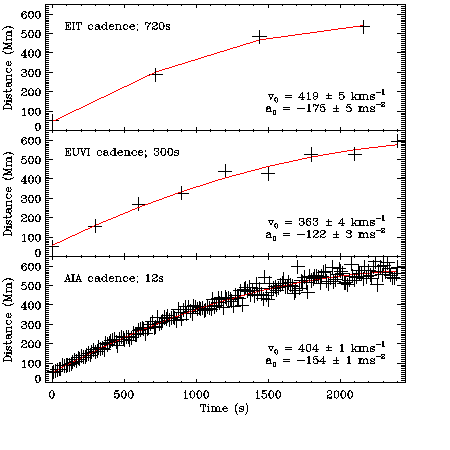
\includegraphics[clip=,trim=0mm 5mm 0mm 0mm,width = 0.5\textwidth]{images/num_diff_cad.pdf}
\caption{Simulated data (crosses) for cadences of 720~s (\emph{top}; comparable to EIT), 300~s  (\emph{middle}; comparable to EUVI) and 12~s  (\emph{bottom}; comparable to AIA). In each case, the fit to the data is shown in red with derived kinematics in the bottom right of each panel.}
\label{fig:num_diff_cad}
\end{center}
\end{figure}

The same data--set was used for each of the panels shown in Figure~\ref{fig:num_diff_cad}, with the cadence varied to best reflect data from \emph{SOHO}/EIT (top panel at 720~s), \emph{STEREO}/EUVI (middle panel at 300~s) and \emph{SDO}/AIA (bottom panel at 12~s). The derived kinematics are given in the bottom right of each panel with the fit to the data shown by the red line. It is immediately apparent that the higher cadence data allows a better fit to the data despite the uncertainty in the data (which was kept at $\pm$5\% of the model for each data--set). This implies that higher cadence data is required to derive the true kinematics of a CBF pulse.

\begin{figure}[!t]
\begin{center}
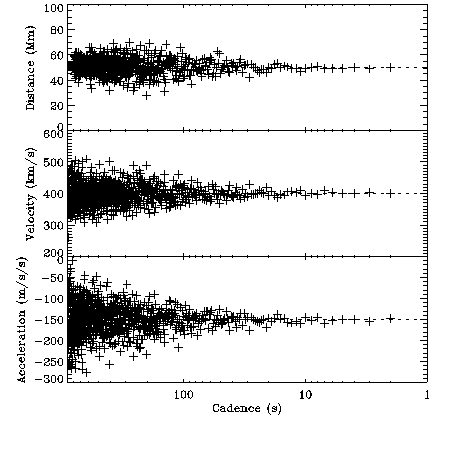
\includegraphics[clip=,trim=0mm 5mm 0mm 0mm,width = 0.5\textwidth]{images/num_diff_vary_cad.pdf}
\caption{Derived kinematics for varying image cadence with $\pm$5\% uncertainty. Distance, velocity and acceleration are shown in the top, middle and bottom panels respectively, with the x--axis shown using logarithmic scaling to highlight the effects of varying the image cadence.}
\label{fig:num_diff_vary_cad}
\end{center}
\end{figure}

The variation in derived kinematics with cadence is shown in Figure~\ref{fig:num_diff_vary_cad} (again for $\pm$5\% uncertainty). As the cadence decreases, the derived velocity and acceleration approach the model values, with the scatter showing a dramatic reduction below $\sim$50~s cadence. These results are consistent with the observations made by both \citet{2008ApJ...680L..81L} and \citet{2009ApJ...707..503M} and show that the effects of image cadence must be accounted for when trying to derive the true kinematics of a CBF pulse.

\begin{figure}[!t]
\begin{center}
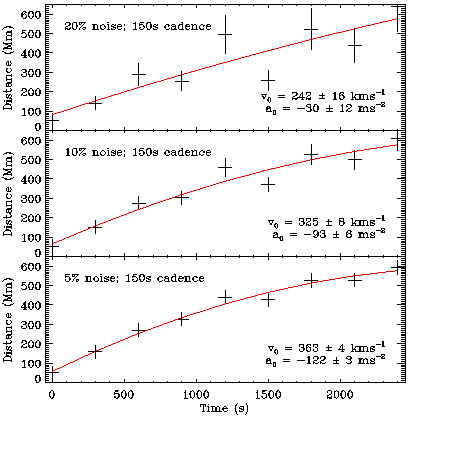
\includegraphics[clip=,trim=0mm 5mm 0mm 0mm,width = 0.5\textwidth]{images/num_diff_noise.pdf}
\caption{Simulated data (crosses) for noise distributions with widths of $\pm$20\% (\emph{top}), $\pm$10\%  (\emph{middle}) and $\pm$5\%  (\emph{bottom}) of the data value. In each case, the fit to the data is shown in red with derived kinematics in the bottom right of each panel.}
\label{fig:num_diff_noise}
\end{center}
\end{figure}

The effects of varying uncertainty in the data were also examined for constant image cadence with the results of this analysis shown in Figures~\ref{fig:num_diff_noise} and \ref{fig:num_diff_vary_noise}. Figure~\ref{fig:num_diff_noise} shows the derived kinematics for the simulated data--set with the top panel showing uncertainties of $\pm$20\%, the middle panel showing uncertainties of $\pm$10\% and the bottom panel showing uncertainties of $\pm$5\%. The variation in uncertainty has a noticeable effect on the derived kinematics in each case, with the acceleration in particular exhibiting significant variation with uncertainty. 

\begin{figure}[!t]
\begin{center}
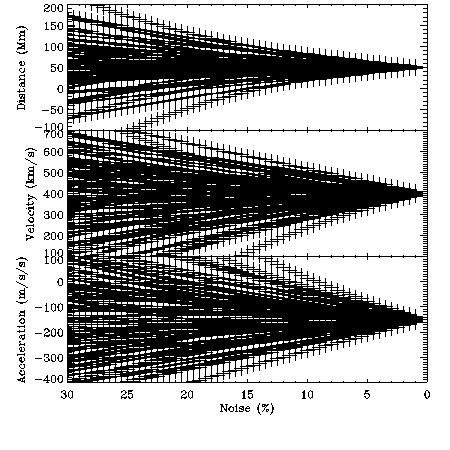
\includegraphics[clip=,trim=0mm 5mm 0mm 0mm,width = 0.5\textwidth]{images/alt_num_diff_vary_noise.pdf}
\caption{Derived kinematics for varying uncertainty at 150~s image cadence. Distance, velocity and acceleration are shown in the top, middle and bottom panels respectively.}
\label{fig:num_diff_vary_noise}
\end{center}
\end{figure}

The variation in the derived kinematics with uncertainty is shown in Figure~\ref{fig:num_diff_vary_noise}, with the variation in offset distance (r$_{0}$), initial velocity (v$_{0}$) and acceleration (a$_{0}$) shown in the top, middle and bottom panels respectively. Some variation is apparent in each case, with the acceleration again showing the strongest variation. The derived kinematics are seen to approach the model kinematics as the noise reduces to 0\% as expected. 

It is clear that the variation in both noise and imaging cadence can strongly influence the derived kinematics of a CBF pulse, while the different numerical differencing techniques do not return accurate estimates of the pulse kinematics. However, it is possible to use a bootstrapping approach to overcome these issues as this is a statistically significant technique that has been optimised for small data-sets such as those typically obtained when studying CBF pulses. 



\section{Bootstrapping}
\label{sect:simul2}

\begin{figure}[!t]
\begin{center}
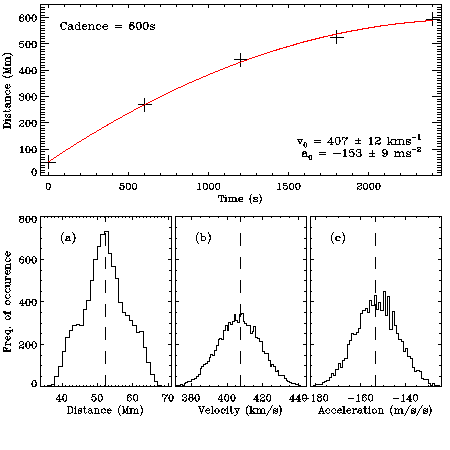
\includegraphics[clip=,trim=0mm 5mm 0mm 0mm,width = 0.49\textwidth]{images/bootstrap.pdf}
\caption{\emph{Top}: Simulated data (asterisks) with bootstrapped fit shown in red and parameters in bottom right. \emph{Bottom}: Histograms showing the distance (a), velocity (b) and acceleration (c) derived using the bootstrapping technique.}
\label{fig:bootstrap}
\end{center}
\end{figure}

Bootstrapping was first proposed by \citet{Efron:1979p1831} as a general interpretation of the jackknife, allowing statistical quantities to be estimated from a limited sample to a high degree of accuracy. In principle this allows a statistical quantity (such as the mean, variance etc.) of a distribution to be estimated using a small sample of measurements from that distribution. The resulting estimates are statistically significant, with statistically defined associated error estimates. 

While there are a number of different bootstrapping techniques, each of which is useful for a different purpose, in this case we will be using the residual resampling technique. Whereas the majority of bootstrapping techniques involve removing one point at random and recalculating the fit to the data, this is inappropriate in this case due to the small sample set available. The residual resampling technique however, does not require data-point removal, making it more appropriate for small data-sets such as those available here.

The residual resampling technique works as follows. The distance-time measurements ($y_i$; $i=1, 2, \ldots, n$) are first fitted using a quadratic equation of the form
\begin{equation}
r(t) = r_0 + v_0 t + \frac{1}{2}a t^2,
\end{equation}
where $r_0$ is the offset distance, $v_0$ is the initial velocity, $a$ is the constant acceleration of the pulse, and $t$ is the time elapsed since the first observation of the disturbance. This yields the fitted values ($\hat{y_{i}}$) and residuals ($\hat{\epsilon}=y_{i} - \hat{y_{i}}$) for each point. The residuals are then randomly ordered and randomly assigned a sign ($1$ or $-1$), before being added to the original fit values to produce a new data set. These new data are then fitted using the same model, with the resulting re-fitted parameters recorded. The process is then repeated a large number of times ($\sim$10\,000).

This has the effect of repeating the fit to slightly varying data a large number of times, allowing a distribution of fit values to be obtained. The mean and standard deviation of this distribution then provide the estimated value and associated error of the parameter. This technique is statistically rigorous and produces a more accurate result than a simple model fit to the given data. 

This technique was applied to the simulated data--set used in Section~\ref{subsect:num_diff} to allow a comparison of the effectiveness of the bootstrapping approach with the numerical differencing techniques. The results of this analysis are shown in Figure~\ref{fig:bootstrap}. The upper panel here shows the simulated data (indicated by the asterisks) with the bootstrapped fit to the data shown by the red line. The kinematics obtained by the bootstrapping approach are given in the bottom right. The bottom panels (a), (b) and (c) show the histograms for the distance, velocity and acceleration parameters respectively. These histograms returned by the bootstrapping approach for each parameter allow a statistical determination of the fit parameters, a fact reflected in the error term for the derived kinematics. 

The kinematics returned by the bootstrapping approach match the model kinematics within one standard deviation, while also producing an accurate estimate with well--defined errors, unlike those of the numerical differencing techniques. It should also be noted that none of the data--points have been removed, unlike the majority of the numerical differencing techniques tested. 

As a result of the simulations carried out to test the different approaches to determining the kinematics of a CBF pulse, the residual resampling bootstrapping technique was chosen as the best method. This fits a model directly to the distance--time measurements, allowing the kinematics of the CBF pulse to be determined to a high degree of accuracy. The kinematics given for each future event studied here therefore reflects the mean value of the bootstrapped distribution, with the associated error given by the standard deviation.

\begin{figure}[!t]
\begin{center}
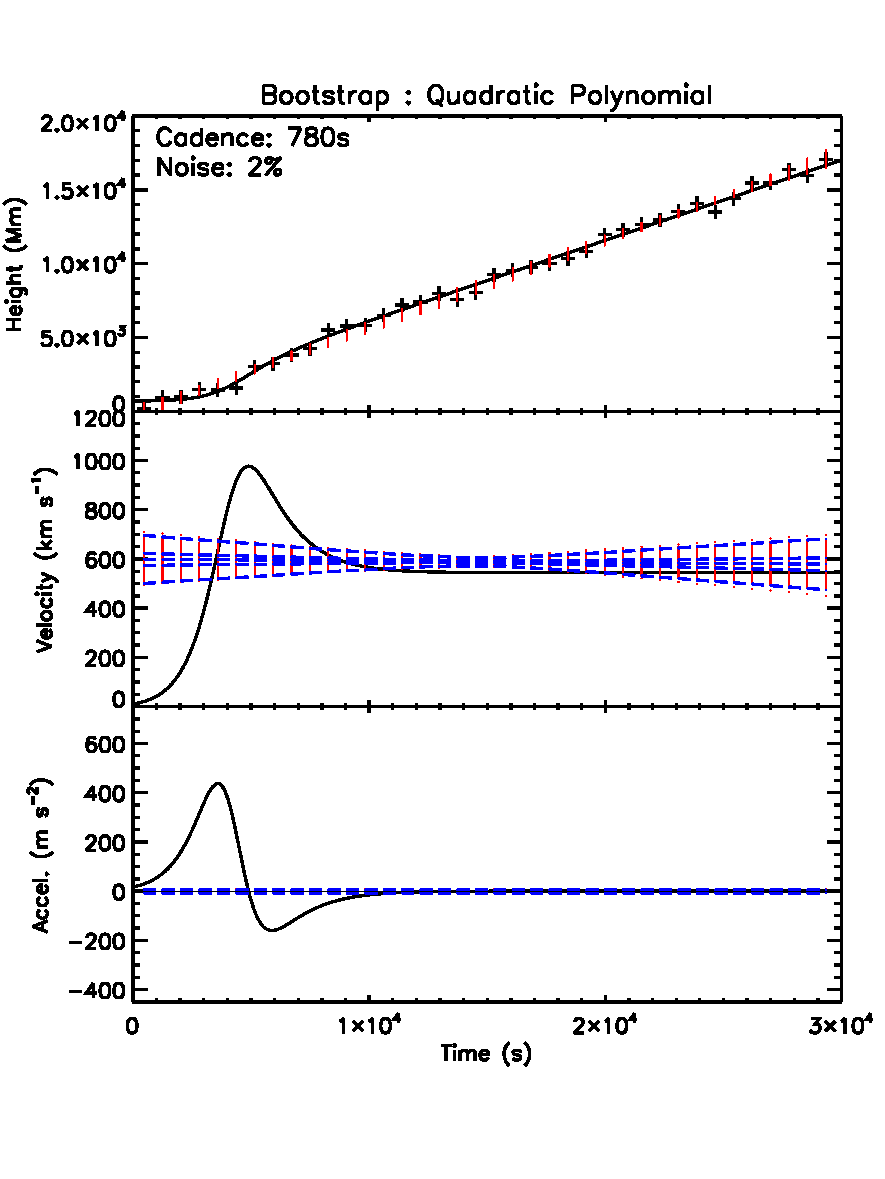
\includegraphics[clip=,trim=0mm 5mm 0mm 0mm,width = 0.49\textwidth]{images/fig_bootstrap_quadratic.pdf}
\caption{\emph{Top}: Simulated data (asterisks) with bootstrapped fit shown in red and parameters in bottom right. \emph{Bottom}: Histograms showing the distance (a), velocity (b) and acceleration (c) derived using the bootstrapping technique.}
\label{fig:bootstrap}
\end{center}
\end{figure}

\begin{figure}[!t]
\begin{center}
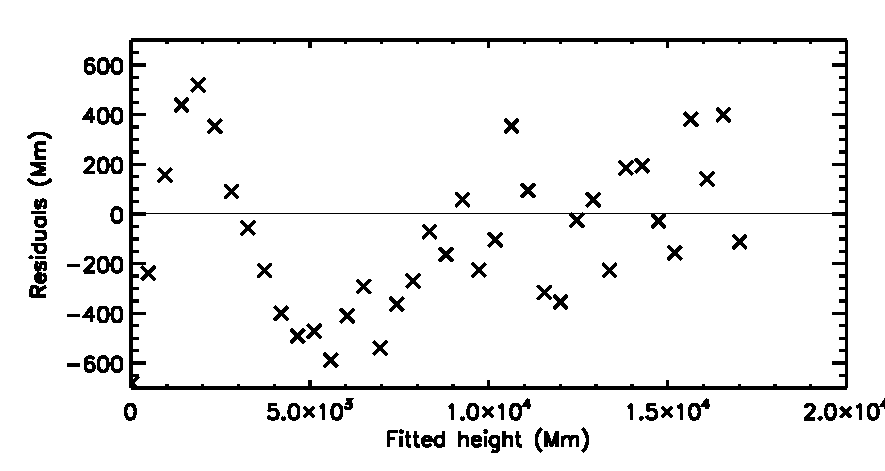
\includegraphics[clip=,trim=0mm 5mm 0mm 0mm,width = 0.49\textwidth]{images/fig_residuals_quadratic.pdf}
\caption{\emph{Top}: Simulated data (asterisks) with bootstrapped fit shown in red and parameters in bottom right. \emph{Bottom}: Histograms showing the distance (a), velocity (b) and acceleration (c) derived using the bootstrapping technique.}
\label{fig:bootstrap}
\end{center}
\end{figure}

\begin{figure}[!t]
\begin{center}
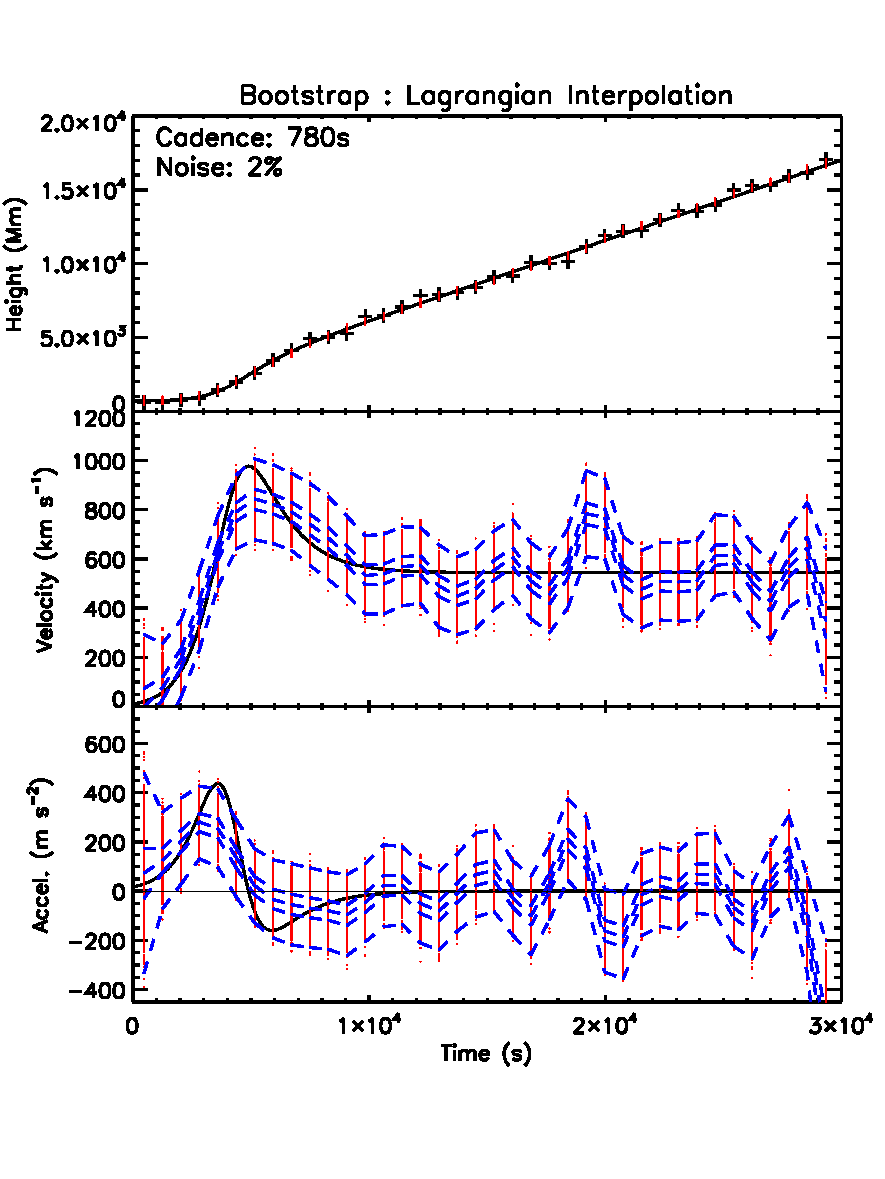
\includegraphics[clip=,trim=0mm 5mm 0mm 0mm,width = 0.49\textwidth]{images/fig_bootstrap_lagrangian.pdf}
\caption{\emph{Top}: Simulated data (asterisks) with bootstrapped fit shown in red and parameters in bottom right. \emph{Bottom}: Histograms showing the distance (a), velocity (b) and acceleration (c) derived using the bootstrapping technique.}
\label{fig:bootstrap}
\end{center}
\end{figure}

\begin{figure}[!t]
\begin{center}
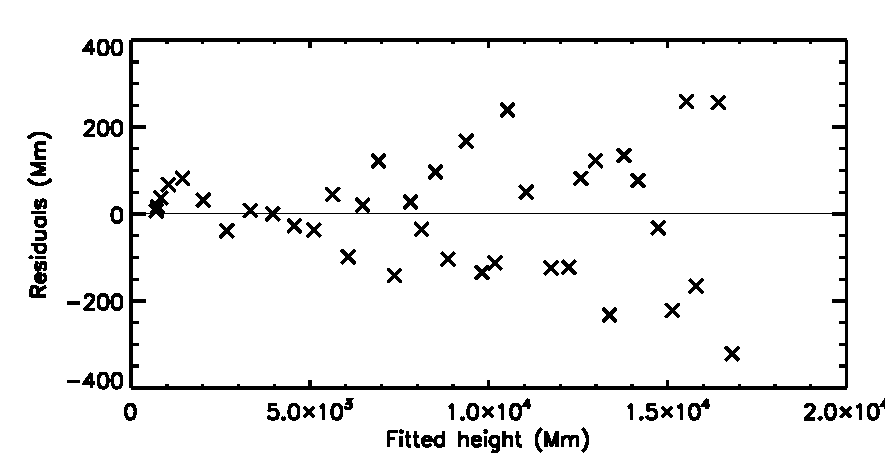
\includegraphics[clip=,trim=0mm 5mm 0mm 0mm,width = 0.49\textwidth]{images/fig_residuals_lagrangian.pdf}
\caption{\emph{Top}: Simulated data (asterisks) with bootstrapped fit shown in red and parameters in bottom right. \emph{Bottom}: Histograms showing the distance (a), velocity (b) and acceleration (c) derived using the bootstrapping technique.}
\label{fig:bootstrap}
\end{center}
\end{figure}

\begin{figure}[!t]
\begin{center}
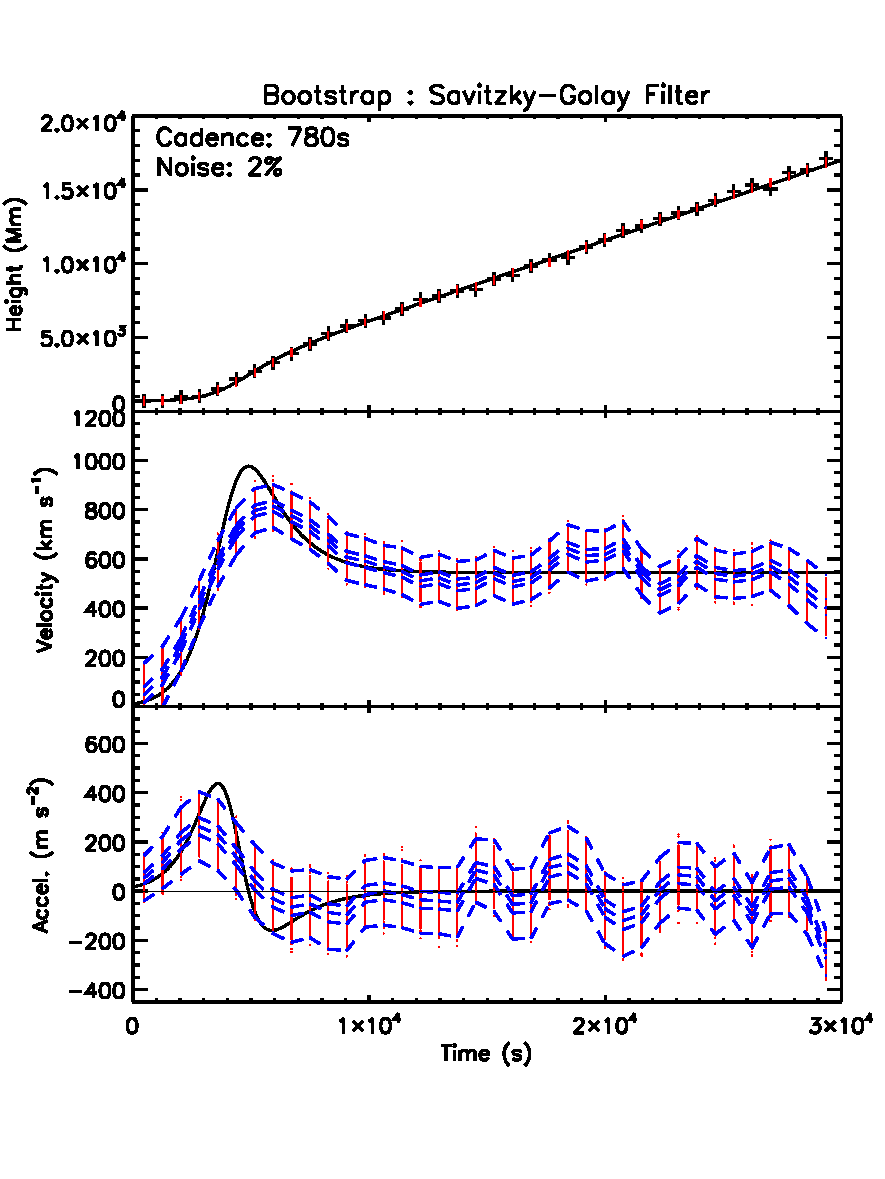
\includegraphics[clip=,trim=0mm 5mm 0mm 0mm,width = 0.49\textwidth]{images/fig_bootstrap_savgol.pdf}
\caption{\emph{Top}: Simulated data (asterisks) with bootstrapped fit shown in red and parameters in bottom right. \emph{Bottom}: Histograms showing the distance (a), velocity (b) and acceleration (c) derived using the bootstrapping technique.}
\label{fig:bootstrap}
\end{center}
\end{figure}

\begin{figure}[!t]
\begin{center}
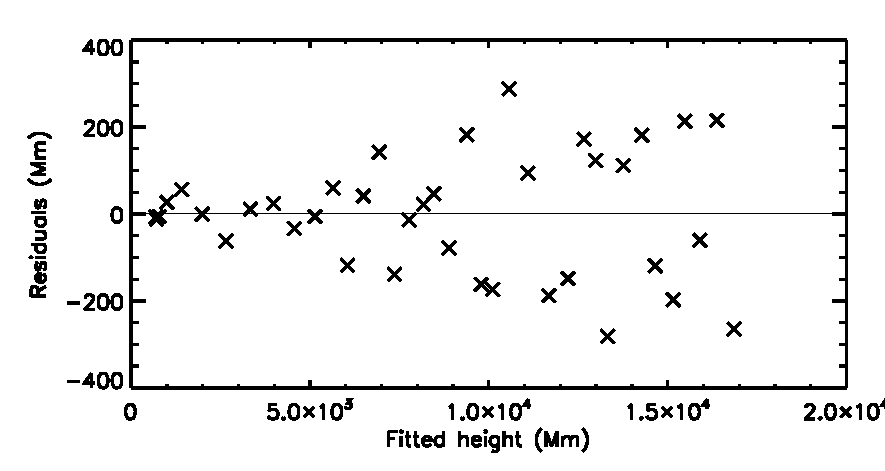
\includegraphics[clip=,trim=0mm 5mm 0mm 0mm,width = 0.49\textwidth]{images/fig_residuals_savgol.pdf}
\caption{\emph{Top}: Simulated data (asterisks) with bootstrapped fit shown in red and parameters in bottom right. \emph{Bottom}: Histograms showing the distance (a), velocity (b) and acceleration (c) derived using the bootstrapping technique.}
\label{fig:bootstrap}
\end{center}
\end{figure}

\section{Case Studies}
\label{sect:case_studies}

\subsection{CORIMP}
\label{subsect:corimp}

\subsection{CorPITA}
\label{subsect:corpita}

\section{Conclusions}
\label{sect:conclusions}


\begin{acknowledgements}
This work is supported by SHINE grant 0962716 and NASA grant NNX08AJ07G to the Institute for Astronomy. The SOHO/LASCO data used here are produced by a consortium of the Naval Research Laboratory (USA), Max-Planck-Institut fuer Aeronomie (Germany), Laboratoire d'Astronomie (France), and the University of Birmingham (UK). SOHO is a project of international cooperation between ESA and NASA. The STEREO/SECCHI project is an international consortium of the Naval Research Laboratory (USA), Lockheed Martin Solar and Astrophysics Lab (USA), NASA Goddard Space Flight Center (USA), Rutherford Appleton Laboratory (UK), University of Birmingham (UK), Max-Planck-Institut f\"{u}r Sonnen-systemforschung (Germany), Centre Spatial de Liege (Belgium), Institut d'Optique Th\'{e}orique et Appliqu\'{e}e (France), and Institut d'Astrophysique Spatiale (France). 
\end{acknowledgements}



\bibliographystyle{apj.bst}
\bibliography{references.bib}  



\end{document}